\begin{figure}[t!]
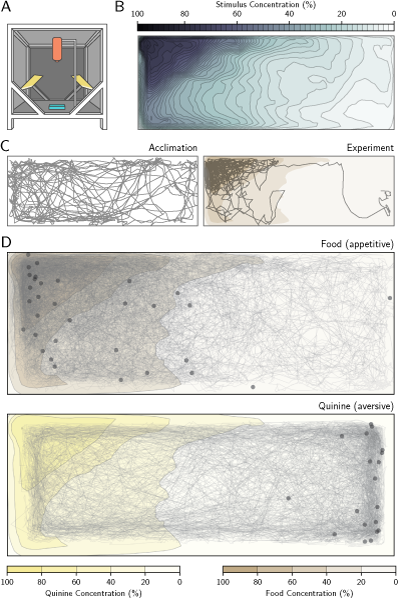
\includegraphics[width=\linewidth]{Figures/images/1.eps}
 \captionof{figure}{\textbf{Quantifying the chemosensory environment in naturalistic larval habitat sizes.} A: Diagram of experimental conditions, adapted from \cite{Bui2018-iq}, including a Basler Scout Machine Vision GigE camera (orange), infrared lighting (yellow) and a behavior arena (blue). B: Chemosensory diffusion map of the behavior arena at the end of the 15 minute experiment. C: Example of an individual larval trajectory during the 15 minute acclimation phase (left). Trajectory of same individual during the 15 minute experiment phase, responding to food added to the left side of the arena (right). D: Trajectory of all starved animals presented with food (top) or quinine (bottom). Although trajectories are shown aggregated into one image, all animals were tested individually. Scatter points show the position of each animal at the end of the experiment.  
 }
 \label{fig:fig1}
\end{figure}